% 图 64.3 —— 由 `checks/emit_hand.py` 自动拼出（probe 精测 + prims2 图元分解）
%%
% ⚠ 这是**稿子不是成品**：跑 `checks/checkhand.py 64.3` 看指标 + 看叠合图。
%%
%% ⚠ 待核：
%   · 本图 probe 报出阴影族 2 个 —— **本脚本不生成阴影**（要照原书手写）；prims2 的 strokes 里可能含阴影线，核对时留意别画重
%   · 可疑字形 1 项（空心圈 ⊙ 常被认成字母 o）—— 见文件末
%%
\documentclass[12pt]{standalone}
\usepackage{fontspec}
\setsansfont{Arial}
\newfontfamily\mfallback{DejaVu Sans}
\usepackage{tikz}
\begin{document}
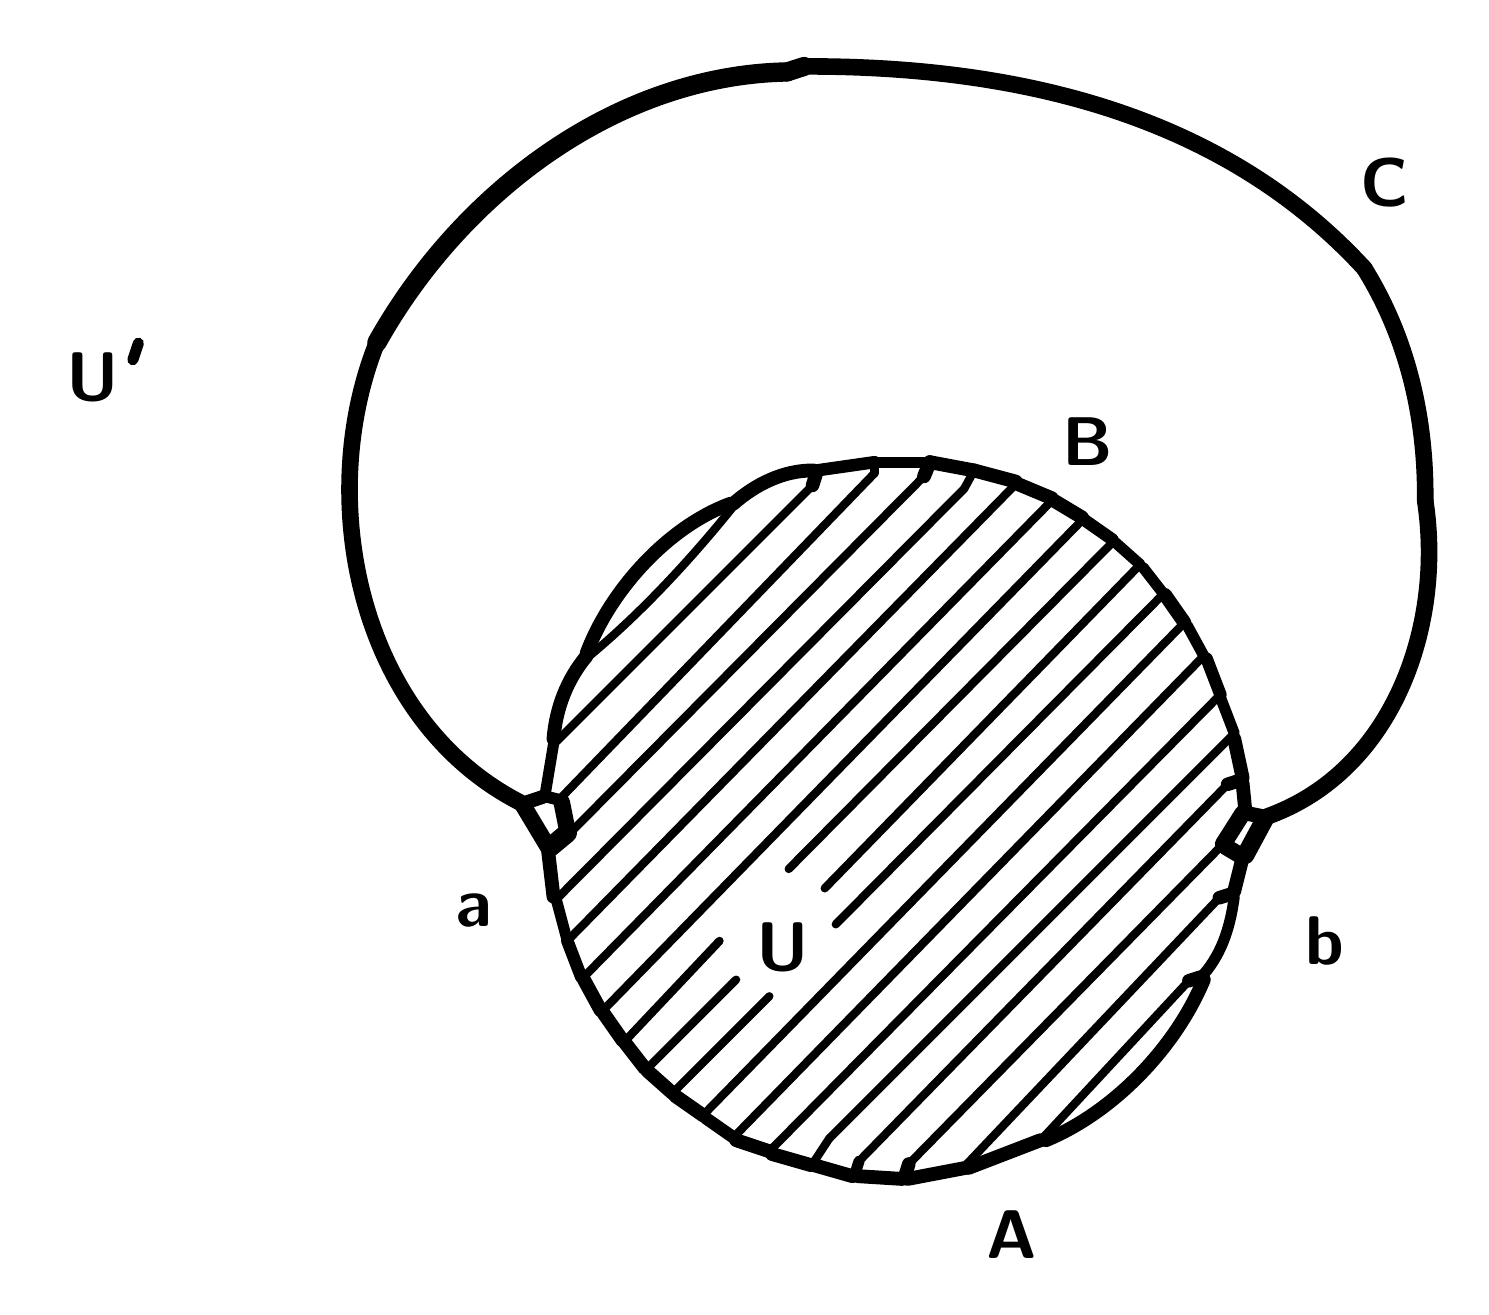
\begin{tikzpicture}[x=1pt, y=-1pt, line width=4.9pt, line cap=round, line join=round]

  %% ════ 直线段（prims2 的 strokes）════
  \draw[line width=4.9pt] (424.0,343.0) -- (419.6,344.4);
  \draw[line width=3.0pt] (419.6,344.4) -- (367.0,401.0);
  \draw[line width=4.5pt] (306.0,157.0) -- (285.0,160.0);
  \draw[line width=5.0pt] (340.0,412.0) -- (366.0,402.0);
  \draw[line width=5.0pt] (436.0,312.0) -- (439.0,300.0);
  \draw[line width=5.0pt] (357.0,164.0) -- (342.0,160.0);
  \draw[line width=4.9pt] (285.0,161.0) -- (283.6,165.4);
  \draw[line width=3.0pt] (283.6,165.4) -- (191.0,258.0);
  \draw[line width=5.0pt] (256.0,402.0) -- (268.0,406.0);
  \draw[line width=6.9pt] (274.4,16.0) -- (280.6,14.0);
  \draw[line width=5.0pt] (370.0,170.0) -- (358.0,165.0);
  \draw[line width=6.0pt] (438.0,299.0) -- (433.0,296.0);
  \draw[line width=3.0pt] (196.0,291.0) -- (323.9,162.1);
  \draw[line width=5.0pt] (323.9,162.1) -- (326.0,157.0);
  \draw[line width=4.5pt] (245.0,394.0) -- (255.0,401.0);
  \draw[line width=3.0pt] (208.0,355.0) -- (380.0,179.0);
  \draw[line width=4.5pt] (200.0,343.0) -- (195.0,330.0);
  \draw[line width=5.0pt] (180.0,280.0) -- (186.0,278.0);
  \draw[line width=6.5pt] (440.0,299.0) -- (447.0,286.0);
  \draw[line width=5.0pt] (234.0,386.0) -- (244.0,393.0);
  \draw[line width=6.0pt] (188.0,296.0) -- (179.0,281.0);
  \draw[line width=4.0pt] (299.0,414.0) -- (300.4,409.6);
  \draw[line width=3.0pt] (300.4,409.6) -- (433.6,273.4);
  \draw[line width=4.9pt] (433.6,273.4) -- (438.0,272.0);
  \draw[line width=4.0pt] (40.0,114.0) -- (38.0,120.0);
  \draw[line width=5.0pt] (284.0,411.0) -- (298.0,415.0);
  \draw[line width=3.0pt] (417.0,216.0) -- (245.0,392.0);
  \draw[line width=5.0pt] (215.0,366.0) -- (208.0,356.0);
  \draw[line width=4.0pt] (195.0,330.0) -- (191.0,315.0);
  \draw[line width=3.0pt] (195.0,330.0) -- (356.0,166.0);
  \draw[line width=5.0pt] (224.0,377.0) -- (233.0,385.0);
  \draw[line width=3.0pt] (288.0,311.0) -- (401.0,195.0);
  \draw[line width=6.0pt] (195.0,290.0) -- (193.0,280.0);
  \draw[line width=5.0pt] (436.0,257.0) -- (439.0,271.0);
  \draw[line width=5.0pt] (418.0,215.0) -- (411.0,205.0);
  \draw[line width=4.0pt] (436.0,255.0) -- (431.0,242.0);
  \draw[line width=4.3pt] (192.0,279.0) -- (188.0,278.0);
  \draw[line width=3.0pt] (256.0,400.0) -- (424.0,228.0);
  \draw[line width=5.0pt] (316.0,416.0) -- (300.0,415.0);
  \draw[line width=4.0pt] (419.0,216.0) -- (425.0,227.0);
  \draw[line width=5.0pt] (216.0,367.0) -- (223.0,376.0);
  \draw[line width=3.0pt] (410.0,205.0) -- (292.0,324.0);
  \draw[line width=5.0pt] (371.0,171.0) -- (381.0,177.0);
  \draw[line width=4.0pt] (326.0,157.0) -- (307.0,157.0);
  \draw[line width=5.0pt] (326.0,157.0) -- (342.0,160.0);
  \draw[line width=5.0pt] (318.0,416.0) -- (339.0,412.0);
  \draw[line width=4.0pt] (187.0,277.0) -- (190.0,259.0);
  \draw[line width=3.0pt] (234.0,384.0) -- (268.0,350.0);
  \draw[line width=3.0pt] (369.0,172.0) -- (201.0,343.0);
  \draw[line width=3.0pt] (306.0,158.0) -- (306.0,161.0);
  \draw[line width=3.0pt] (306.0,161.0) -- (193.0,278.0);
  \draw[line width=5.0pt] (439.0,273.0) -- (440.0,283.0);
  \draw[line width=5.0pt] (190.0,314.0) -- (188.0,297.0);
  \draw[line width=4.0pt] (402.0,194.0) -- (393.0,186.0);
  \draw[line width=3.0pt] (342.0,160.0) -- (338.4,166.6);
  \draw[line width=3.0pt] (338.4,166.6) -- (192.0,314.0);
  \draw[line width=4.0pt] (403.0,195.0) -- (410.0,204.0);
  \draw[line width=4.5pt] (392.0,185.0) -- (382.0,178.0);
  \draw[line width=5.0pt] (283.0,411.0) -- (269.0,407.0);
  \draw[line width=4.9pt] (317.0,415.0) -- (318.4,410.6);
  \draw[line width=3.0pt] (318.4,410.6) -- (431.0,296.0);
  \draw[line width=7.0pt] (189.0,296.0) -- (195.0,291.0);
  \draw[line width=3.0pt] (284.0,410.0) -- (289.7,401.3);
  \draw[line width=3.0pt] (289.7,401.3) -- (435.0,256.0);
  \draw[line width=5.0pt] (207.0,355.0) -- (201.0,344.0);
  \draw[line width=6.0pt] (439.0,284.0) -- (432.0,295.0);
  \draw[line width=4.5pt] (431.0,241.0) -- (426.0,228.0);
  \draw[line width=5.3pt] (441.0,284.0) -- (446.0,285.0);
  \draw[line width=3.0pt] (275.0,304.0) -- (391.0,187.0);
  \draw[line width=3.0pt] (256.0,344.0) -- (224.0,376.0);
  \draw[line width=3.0pt] (269.0,405.0) -- (430.0,242.0);
  \draw[line width=3.0pt] (216.0,366.0) -- (250.0,330.0);
  \draw[line width=3.0pt] (339.0,411.0) -- (430.6,314.4);
  \draw[line width=4.9pt] (430.6,314.4) -- (435.0,313.0);

  %% ════ 曲线（prims2 的 curves —— 三段式，坐标同为 (y,x)）════
  \draw[line width=5.0pt] (284.0,160.0) .. controls (273.1,159.9) and (263.0,165.0) .. (255.0,172.0);
  \draw[line width=4.0pt] (425.0,342.0) .. controls (431.9,334.0) and (434.7,324.0) .. (436.0,314.0);
  \draw[line width=3.0pt] (203.0,227.0) .. controls (221.6,211.6) and (239.8,191.9) .. (255.0,173.0);
  \draw[line width=6.0pt] (178.0,280.0) .. controls (119.7,250.1) and (103.4,170.6) .. (126.2,113.8);
  \draw[line width=7.0pt] (126.2,113.8) .. controls (156.2,60.1) and (212.2,17.2) .. (274.4,16.0);
  \draw[line width=6.0pt] (280.6,14.0) .. controls (355.5,13.8) and (430.8,30.2) .. (483.0,87.0);
  \draw[line width=6.0pt] (483.0,87.0) .. controls (498.5,112.0) and (505.3,140.7) .. (505.0,171.0);
  \draw[line width=6.0pt] (505.0,171.0) .. controls (511.8,215.4) and (493.9,268.5) .. (448.0,285.0);
  \draw[line width=5.0pt] (202.0,226.0) .. controls (210.5,203.4) and (231.3,180.3) .. (254.0,172.0);
  \draw[line width=5.0pt] (202.0,227.0) .. controls (194.8,235.6) and (190.9,246.0) .. (190.0,257.0);
  \draw[line width=5.0pt] (425.0,344.0) .. controls (414.8,368.5) and (392.5,391.8) .. (368.0,402.0);

  %% ════ 标签（probe 直接给的 \node 行）════
  %% ⚠ 全部补了 fill=white：文字在最上层，否则与曲线交叉干扰
     \node[anchor=center,inner sep=0pt,fill=white,font=\fontsize{32.2}{40.3}\selectfont] at (490.3,55.8) {\textsf{\textbf{\textit{C}}}};   % box(479,44,21,23)
     \node[anchor=center,inner sep=0pt,fill=white,font=\fontsize{28.9}{36.1}\selectfont] at (23.5,126.2) {\textsf{\textbf{\textit{U}}}};   % box(14,114,19,22)
     \node[anchor=center,inner sep=0pt,fill=white,font=\fontsize{29.6}{37.0}\selectfont] at (383.2,149.5) {\textsf{\textbf{\textit{B}}}};   % box(372,138,19,22)
     \node[anchor=center,inner sep=0pt,fill=white,font=\fontsize{31.0}{38.7}\selectfont] at (161.5,319.0) {\textsf{\textbf{\textit{a}}}};   % box(153,309,15,17)
     \node[anchor=center,inner sep=0pt,fill=white,font=\fontsize{30.7}{38.3}\selectfont] at (468.8,329.8) {\textsf{\textbf{\textit{b}}}};   % box(459,317,17,23)
     \node[anchor=center,inner sep=0pt,fill=white,font=\fontsize{29.6}{37.0}\selectfont] at (273.0,332.2) {\textsf{\textbf{\textit{U}}}};   % box(263,320,20,22)
     \node[anchor=center,inner sep=0pt,fill=white,font=\fontsize{28.1}{35.2}\selectfont] at (355.6,436.0) {\textsf{\textbf{\textit{A}}}};   % box(344,425,18,21)

  % 钉死画布：否则超出的图元/控制点会把页面撑大，1:1 回比就失准
  \pgfresetboundingbox
  \path[use as bounding box] (0,0) rectangle (518,455);
\end{tikzpicture}
\end{document}

% ⚠ 待核清单（probe 拿不准，人眼过一遍）：
%   · 未识别/跳过：⑤ 跳过/未识别的字形
